\documentclass[a4paper,12pt]{report} 
\usepackage[utf8x]{inputenc}
\usepackage[french]{babel}
\usepackage{mathtools}
\usepackage{amsmath}
\usepackage{amsfonts}
\usepackage{amssymb}
\usepackage{textcomp}
\usepackage[nointegrals]{wasysym}			% Collection de symboles mathématiques
\usepackage{multicol}					% Pour utiliser \hfill
\usepackage{ifthen}
\usepackage{tabularx}	 				% Gestion avancée des tableaux
%\usepackage{cleveref}

\usepackage{enumitem}
\usepackage{wrapfig}
%\usepackage[squaren]{SIunits}
%\usepackage[T1]{fontenc}				% Indispendable, présent dans tous les codes exemples
\usepackage[linkcolor=DarkGreen,colorlinks=true, citecolor= DarkGreen, urlcolor=MidnightBlue]{hyperref} 	% Hyper ref
\usepackage{listings}					% Pour citer du code
\usepackage[justification=centering]{caption}
\usepackage{sistyle} 
\usepackage{numprint}
\usepackage{wrapfig}
\usepackage{cite}	
\usepackage{url} 					% Pour citer les sites internet dans la
%\usepackage{cleveref}
\usepackage{setspace}

\usepackage{graphicx}		 			% Inclusion des figures
\graphicspath{{./pic/}, {./../figures/ML}}
\usepackage[svgnames]{xcolor}			%https://www.latextemplates.com/svgnames-colors

%%% Commandes utiles définies
\newcommand{\argmin}{\mathop{\mathrm{argmin}}}

\newcommand{\bepar}[1]{
	\left( #1 \right)  
}

\newcommand{\becro}[1]{
	\left[ #1 \right]  
}

\newcommand{\rbk}[1]{\color{red}\textit{#1} \color{black}  
}

\usepackage{listings}					% Pour citer du code
%%%%%%%%%%%%%%%%%%%
%%% Élément pour citer des codes %%%
\lstset{
language=Python,
basicstyle=\ttfamily\bfseries\small, %
identifierstyle=\bfseries\color{black}, %
keywordstyle=\color{blue}, %
stringstyle=\color{black!90}, %
commentstyle=\it\color{black!70}, %
columns=flexible, %
tabsize=4, %
extendedchars=true, %
showspaces=false, %
showstringspaces=false, % %
numberstyle=\small, %
breaklines=true, %
breakautoindent=true, %
captionpos=b,
otherkeywords={cross_val_score},
keywords=[0]{cv},
keywordstyle=[0]{\color{red}},
}
%%%%%%%%%%%%%%%%%%%%%
%\usepackage{multicol}
%\usepackage{etoolbox}
%\patchcmd{\thebibliography}{\section*{\refname}}
%    {\begin{multicols}{2}[\section*{\refname}]}{}{}
%\patchcmd{\endthebibliography}{\endlist}{\endlist\end{multicols}}{}{}
\usepackage[authoryear]{natbib}

\usepackage{geometry}
\geometry{hmargin=2cm, vmargin=2cm}

%%%%%%%%%%%%%%%%%%%%
%%% Couleurs %%%
\xdefinecolor{brick}{named}{DarkRed}
\xdefinecolor{navy}{named}{Navy}
\xdefinecolor{midblue}{named}{MidnightBlue}
\xdefinecolor{dsb}{named}{DarkSlateGray}
\xdefinecolor{dgreen}{named}{DarkGreen}

%%% 	Raccourcis 	%%%
\newcommand{\keps}{$k-\varepsilon$}
\newcommand\bk{\color{black}}
\newcommand\brick{\color{brick}}
\newcommand\navy{\color{navy}}
\newcommand\midblue{\color{midblue}}
\newcommand\dsb{\color{dsb}}
\newcommand{\dgreen}{\color{dgreen}}
\newcommand\red{\color{red}}

%%%%%%%% Cigles
\newcommand{\rap}{par rapport}
\newcommand{\cad}{c'est-à-dire}
\newcommand{\vav}{vis-à-vis}

%%%%%%%% Autres

%%%%%%%%%%%%%%%%%%%
% Syntax: \colorboxed[<color model>]{<color specification>}{<math formula>}
\newcommand*{\colorboxed}{}
\def\colorboxed#1#{%
  \colorboxedAux{#1}%
}
\newcommand*{\colorboxedAux}[3]{%
  % #1: optional argument for color model
  % #2: color specification
  % #3: formula
  \begingroup
    \colorlet{cb@saved}{.}%
    \color#1{#2}%
    \boxed{%
      \color{cb@saved}%
      #3%
    }%
  \endgroup
}
\title{\navy \textbf{Notes Machine Learning} \color{black}}%%%%%%%%%%%%%%%%%%%%
\date{}

\renewcommand{\sectionmark}[1]{\markright{#1}}
\usepackage{fancyhdr}
\pagestyle{fancy}
\lhead{\textbf{Nathaniel} \brick \textbf{\textsc{Saura}}}
\rhead{\markright}
\cfoot{\thepage}
\renewcommand{\headrulewidth}{0.4pt}

\numberwithin{equation}{section} %%%% To count the equation like Section.Number

\begin{document}
\maketitle
\chapter{Présentation}
Réseaux de neurones : ensemble d'opération mathématiques visant à ajuster les hyperparamètres du réseaux pour associer la meilleure sortie à une entrée donnée. \\
Deux phases : une phase d'entraînement pour laquelle les entrées et les sorties sont fournies à l'algorithme et une phase de prédiction ou seule les entrées sont fournies.\\
Pendant la phase d'entraînement les poids et biais (hyperparamètres) liant chacune des couches cachées entre elles, sont ajustés de sorte à minimiser l'erreur commise entre la prédiction et la sortie espérée, à chaque époque.\\

\noindent L'équation que l'on cherche à modéliser est l'équation de Burgers 1D diffusif (VBE):
\begin{equation*}
\frac{\partial u}{\partial t} + u \frac{\partial u}{\partial x} = \nu \frac{\partial^2 u}{\partial x^2} 
\end{equation*}

Nous cherchons à statuer s'il était possible de prédire la valeur du champ de vitesse à chaque itération temporelle avec un réseaux de neurones \textit{i.e.} savoir si on pouvait écrire 
\begin{equation*}
u^{n+1} = \mathcal{F}\bepar{u^n}	
\end{equation*}
Avec $\mathcal{F}$ une fonctionnelle dépendant d'information provenant du champ de viteses au temps $n$ estimée à partir d'un réseau de neurones.\\
Ici on teste différents architectures et différentes matrice d'entrées $X$.\\
On testera aussi selon ces architectures et ces matrices d'entrées la méthode de Bootstrapping.

\pagebreak

\section*{Architecture N3}
L'ensemble des architecture ont été entraînées sur la résolution des conditions initiales présentées figure \eqref{ci}. La résolution se fait en utilisant un schéma de Lax-Wendroff (classique pour simuler les chocs). Les champs de vitesse pour toutes les 60 itérations sont calculées puis enregistrées. Les matrices $X$ et $y$ sont construits comme suit : selon le type d'entrées considéré, on ajoute ligne par ligne, dans la matrice des entrées $X$, les grandeurs voulues de l'itération $n$ dans une maille relative au $j$-ème point, $\forall j \in \ \{ 0, N_x-1 \}$, et on y fait correspondre  la valeur du champ de vitesse de l'itération $n+1$ dans la matrice $y$. Les conditions sont supposées périodiques.\\
Les matrices ont donc les tailles suivantes : $$\dim\left(X \right) = (n_{\text{init}} \times (N_x - 2) \times (\text{itmax} - 1),\ n_{\text{features}}) $$
											  $$ \dim \left(y \right) = (n_{\text{init}} \times (N_x - 2) \times (\text{itmax} - 1), \ 1 ) $$

\begin{figure}[!ht]
\centering
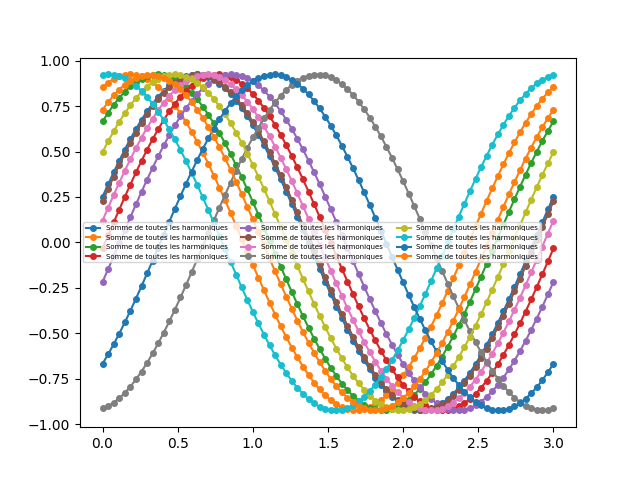
\includegraphics[scale=1]{/CI.png}
\caption{Conditions initiales de cas pour la construction du train set. Toutes ces situations sont résolues à partir d'un solver Lax-Wendroff pour 60 itérations. Les champs de vitesses pour toutes les itérations sont agglomérés dans une matrice $X$ la cible correspondante est enregistrée dans une matrice $y$}
\label{ci}
\end{figure}

\subsection*{X tenant compte de la dérivée du point courant}
On construit $X$ comme suit : 
\begin{equation}
\left[ \begin{array}{c} 
		. \\
		. \\
		u_{j-1}^n, u_j^n, u_{j+1}^n, \frac{u_{j+1}^n - u_{j-1}^n}{2 \Delta x} \\
		. \\
		.  
	   \end{array}
\right]
\end{equation}



\end{document}